
As seen before in sec \ref{sec:tau_lepton}, when a $\tau$ is produced in a collision, it can decay into several different final states.
Hadronic final states, denoted \tauh, represent about 65\% of tau decays.
These hadronic final states are characterized by one or three charged hadrons with or without \pizero .

But similar particles can be reconstructed from other processes and decays, such as QCD jets.
Since these QCD jets greatly outnumber \tauh in the final states of proton-proton collisions at the LHC, \tauh identification algorithms have be designed in CMS to reject QCD jets as much as possible while keeping a \tauh identification efficiency somewhere between 35\% and 70\%, depending on the purity needed by the analyses. Identification is performed on a jet basis, meaning algorithms classifies all reconstructed jets as either background, meaning QCD jets, or signal, meaning \tauh decay products.

These standard \tauh identification algorithms, as will be presented in section \ref{sec:std_tau_id}, have reached excellent performance thanks to the use of particle-flow reconstruction but do not use its full potential.

Deep learning algorithms, that will be introduced in section \ref{sec:NN}, have shown an ability to use available information as efficiently as possible for the task they are trained for. In the field of particle physics, for example, their use in heavy flavour jet-tagging \cite{btagging_NN} has shown significant improvements over previously used techniques. These networks show best results when their design, or architecture, helps simplify the task at hand. New architectures specifically intended for high energy proton-proton collisions have shown promising results. One such architecture is the Recursive Neural Network (RecNN) \cite{Louppe:2017ipp} used to identify boosted jets originating from hadronically decaying W bosons. This could be adapted to similar tasks, such as \tauh identification. The section \ref{sec:RecNN} will detail this adaptation to the \tauh identification task and the improvements from the original design. But machine learning techniques such as the RecNN need to be trained on well identified data. The CMS simulated data offers such a possibility, as the provenance of the reconstructed jets can be easily found. A chunk of these datasets is also going to be used to compare the performance of both the standard and the RecNN approach. The specificities of the selected datasets are then first going to be presented in section \ref{sec:NN_datasets}, as it introduces the context of the study.

\section{Simulation of QCD jets and hadronic $\tau$ decays}
\label{sec:NN_datasets}

In order to compare the several classification methods, their performance is expressed in terms of signal efficiency and background rejection. To quantify these, and to provide a training set for our deep learning algorithm, datasets of QCD jets and hadronic tau decays have been selected from the simulated CMS datasets that were introduced in \ref{sec:cms_physics_event_generation}. Instead of simulating isolated QCD jets and \tauh separately, entire collision events are used as they provide a realistic environment similar to the one in which the classifier will be used.

Selected processes leading to \tauh and QCD jets in the final state are detailed in table \ref{tab:NN_b_s_diff}. QCD jets are obtained from QCD multijet events in which true \tauh are extremely rare, while \tauh are taken from events with true taus in the final state (MSSM $H\rightarrow \tau\tau$, DY $Z\rightarrow \tau\tau$).

% As seen in sec \ref{sec:cms_physics_event_reconstruction}, after particle-detector interaction is simulated, reconstruction will undergo the exact same algorithms in both real data in simulation, meaning both classical and, if proven to be useful, deep-learning based algorithms identification algorithms, the reconstruction steps that precede identification will be detailed in sub-section \ref{sec:NN_datasets_pf}. Although to be able to quantify both methods in terms of background rejection and signal identification, only simulation will be used to compare.

The proton-proton collision events are generated with PYTHIA 8 \cite{SJOSTRAND2008852}, and are then processed by the CMS GEANT4 simulation, as detailed in section \ref{sec:cms_physics_event_generation}. The generation-level information is kept and will be referred to as gen level. All the information coming out of the detector simulation is fed to the CMS reconstruction algorithms, where the particle flow algorithm provides the list of reconstructed stable particles. Higher-level objects such as jets, are reconstructed by combining these particles using the clustering algorithms introduced in \ref{sec:jet_clustering}.

At this point most reconstructed particles, isolated or not, are part of a reconstructed jet. Since the role of the studied classifiers is to classify reconstructed jets as QCD jets or \tauh decays, the information is split on a single jet basis.

A reconstructed jet is defined as signal if it is selected from the genuine tau samples, and as background if selected from the QCD multijet samples. To ensure purity, some extra cuts are applied, these cuts can be found in table \ref{tab:NN_b_s_diff}.

The matching between reconstructed jets and gen-level \tauh is done by ensuring their respective directions are aligned, meaning that the distance separating their orientation in the ($\eta ,\phi$) plane is less than $0.1$.


\begin{table}[ht]
    \caption{Provenance and cuts applied to reconstructed jets defining signal and background.}
    \centering
    \begin{adjustbox}{max width=\textwidth}
    \begin{tabular}{c||c|c}
        & \tauh (signal) & QCD jets (background) \\
        \hline \hline
        \multirow{3}{*}{Hard processes} & SUSY ggH $\rightarrow\tau\tau$ & \multirow{3}{*}{\begin{minipage}{0.4\textwidth}QCD multijets samples ordered by \pt : 15-30, 30-50, 50-80, 80-120, 120-170, 170-300 \end{minipage}} \\
        \cline{2-2}
         & SUSY bbH to $\rightarrow\tau\tau$ & \\
        \cline{2-2}
         & DY to tautau & \\
        \hline
        phase-space cuts & \multicolumn{2}{c}{$20<\pt<100 \text{ and } |\eta|<0.8$}\\
        \hline
        specific extra cuts & matched with gen-level \tauh & any \\
        \hline
    \end{tabular}
    \end{adjustbox}
    \label{tab:NN_b_s_diff}
\end{table}

\section{The standard CMS hadronic $\tau$ decays identification}
\label{sec:std_tau_id}
\subsection{Decay mode finding}

First, the particles of the reconstructed jet are fed as input to the hadrons-plus-strip (HPS) algorithm \cite{tauh_reconstruction} to reconstruct and identify \tauh candidates. A first selection is the requirement that reconstructed jets have $\pt > 14\,\mathrm{GeV}$ and $|\eta| < 2.5$.
The constituent particles are combined into \tauh candidates compatible with one of the main $\tau$ decay modes, $\tau^- \rightarrow h^- \nu_\tau$, $\tau^- \rightarrow h^- \pizero \nu_\tau$, $\tau^- \rightarrow h^- \pizero \pizero \nu_\tau$, $\tau^- \rightarrow h^- h^+ h^- \nu_\tau$, and charge conjugates. The decay mode $\tau^- \rightarrow h^- h^+ h^- \pizero \nu_\tau$ is not considered owing to its relatively small branching fraction and high contamination from quark and gluon jets.

The \pizero produced in some decay modes have a mean life of about $9 \times 10^{-17}\,\mathrm{s}$ and about $99\%$ of their decays lead to two photons. Because of the large amount of material in the tracker, illustrated in figure \ref{fig:tracker_material}, photons often convert before reaching the ECAL. The resulting electrons and positrons can be identified as such by the PF algorithm or, in the case their track is not reconstructed, as photons displaced along the $\phi$ direction because their trajectory is bent by the magnetic field.
These neutral pions are therefore obtained by adding iteratively reconstructed photons and electrons located in a strip of size $0.05 \times 0.20$ in the ($\eta$,$\phi$) plane:
\begin{itemize}
    \item Every reconstructed electrons and photons of $\pt > 0.5\,\mathrm{GeV}$ in the strip are added iteratively from highest to lowest \pt.
    \item At every step, the position of the center of the strip is re-computed as a \pt-weighted average of the position of all constituents.
    \item Any electron or photon not included in an existing strip is used as seed to another new strip.
\end{itemize}

\tauh candidates are then formed by creating all combinations of either one or three charged-particle and up to two strips in the jet.
Each \tauh candidate is then required to have a mass compatible with its decay mode and to have unit charge.
Collimation of the products are ensured by requiring all charged hadrons and neutral pions to be within a circle of radius $\Delta R = (2.8\,\mathrm{GeV})/\pt$ in the ($\eta$,$\phi$), which is called the signal cone.
The size of the signal cone is, however, not allowed to increase above 0.1 at low \pt, nor to decrease below 0.05 at high \pt. It decreases with \pt to account for the boost of the $\tau$ decay products. Finally, the highest \pt selected \tauh candidate in a given jet is retained. The four-momentum of the \tauh candidate is determined by summing the four-momenta of its constituent particles.

\subsection{Isolation}


\tauh candidates reconstructed from QCD jets are likely to be surrounded by other particles coming from the jet.
Isolation is therefore a powerful way to reject background QCD jets.

Two approaches are available : cut-based and multi-variate.

\paragraph{Cut-based} Isolation is computed from the \pt sum of charged particles and photons with $\pt > 0.5$ GeV within an isolation cone of $dR=0.5$ centered around the \tauh direction, excluding particles used to form the \tauh candidate. In order to mitigate pileup contribution, tracks associated to the considered charged particles are required to be compatible with the \tauh production vertex within a distance $\Delta z < 0.2\,\mathrm{cm}$ and $\Delta r < 0.03\,\mathrm{cm}$. The contribution from pileup is estimated as $\Delta \beta$ calculated from the contribution of charged displaced particles and removed as
\begin{equation}
    I_{\tau} = \sum_{charged, \Delta z<0.2 cm} \pt + max \Big\{ 0, \sum_{\gamma} \pt - \Delta\beta \Big\} \msep
    \label{eq:isolation}
\end{equation}
\begin{equation}
    \Delta \beta = 0.46 \sum_{charged,\Delta z>0.2 cm} \pt \mend
\end{equation}
Working points are defined by the thresholds on the value taken by the isolation defined in equation \ref{eq:isolation}. Usual working points such as loose, medium, tight are thresholds are 2.0, 1.0 and $0.8\,\mathrm{GeV}$ respectively.

\paragraph{Multi-variate} This method is based on decision trees. These are machine learning techniques that rely on finding the best successive cuts on the available variables to separate signal and background in a training set. Boosting is a method of combining many weakly classifying trees into a strong classifier. A BDT is trained on an appropriate choice of isolation variables to give best separation between QCD jets and \tauh : 
    \begin{itemize}
        \item charged- and neutral-particle isolation sums defined as in eq \ref{eq:isolation}.
        \item The reconstructed decay mode.
        \item the transverse impact parameter $d_0$ of the leading tack of the \tauh candidate and its significance $d_0 / \sigma_{d_0}$
        \item the distance between the $\tau$ production and decay vertices, $|\Vec{r}_{SV} - \Vec{r}_{PV}|$, and its significance $|\Vec{r}_{SV} - \Vec{r}_{PV}|/\sigma_{|\Vec{r}_{SV} - \Vec{r}_{PV}|}$, along with a flag indicating whether a decay vertex has successfully been reconstructed for a given \tauh candidate. The positions of the vertices, $\Vec{r}_{SV}$ and $\Vec{r}_{PV}$, are reconstructed using the adaptive vertex-fitter algorithm \cite{Waltenberger_2007}.
        \item More details on the variables can be found in \cite{tauh_reconstruction}.
    \end{itemize}

\subsection{Anti-leptons discriminants}

Electrons and muons can easily be misidentified as \tauh, particularly in the $h^{\pm}$ decay mode. Electrons radiating a bremsstrahlung photon that subsequently converts may also get reconstructed in the $h^{\pm}\pizero$ decay mode. Therefore discriminants have been developed to separate such leptons decays from real \tauh decay products.

Electrons are rejected by a BDT using observables that quantify the distribution in energy depositions in the ECAL and HCAL, in combination with observables sensitive to the amount of bremsstrahlung emitted along the leading track. The BDT also uses observables sensitive to the overall particle multiplicity, to distinguish electromagnetic from hadronic showers.
All these variables are listed in \cite{tauh_reconstruction}.
    
Muons are rejected by requiring that no track segments are found in at least two muon stations within a cone of size $\Delta R = 0.3$ around the \tauh direction. \tauh candidates are also rejected when the sum of the energies in the ECAL and HCAL corresponds to less than 20\% of the momentum of their leading track.
    % \item Electrons are discriminated with a BDT using the following variables:
    % \begin{itemize}
    %     \item Electromagnetic energy fraction of the charged particles and photons that constitue the \tauh candidate : $E_{ECAL}/(E_{ECAL} + E_{HCAL})$.
    %     \item $E_{ECAL}/p$ and $E_{HCAL}/p$, defined as rations of ECAL and HCAL energies relative to the momentum of the leading charged-particle track of the \tauh candidate.
    %     \item $\sqrt{\sum(\Delta \eta)^2 \pt^{\gamma}}$ and $\sqrt{\sum(\Delta \phi)^2 \pt^{\gamma}}$, the respective \pt-weighted (in GeV) root-mean-square distances in $\eta$ and $\phi$ between the photons in any strip and the leading charged particle.
    %     \item $\sum E_{\gamma}/E_{\tau}$, the fraction of \tauh energy carried by photons.
    %     \item $F_{brem} = (p_{in}-p_{out})/p_{in}$, where $p_{in}$ and $p_{out}$ are measured by the curvature of the leading track, reconstructed using the GSF algorithm, at the innermost and outermost positions of the tracker.
    %     \item $(E_e + \sum E_{\gamma})/ p_{in}$, the ratio between the total ECAL energy and the ineer track momentum. Thr quantities $E_e$ and $E_{\gamma}$ represent the energies of the electron cluster and of bremsstrahlung photons, respectively. $\sum E_{gamma}$ is reconstructed by summin the energy depositions in ECAL clusters located along the tangent to the GSF track.
    %     \item $\sum E_{\gamma}/(p_{in}-p_{out})$, the ratio of energies of the bremsstrahlung photons measured in the ECAL and in the tracker.
    %     \item $m_{\tauh}$, the mass of the \tauh candidate.
    %     \item $$
    % \end{itemize}

\subsection{Performance}


\begin{figure}
    \centering
    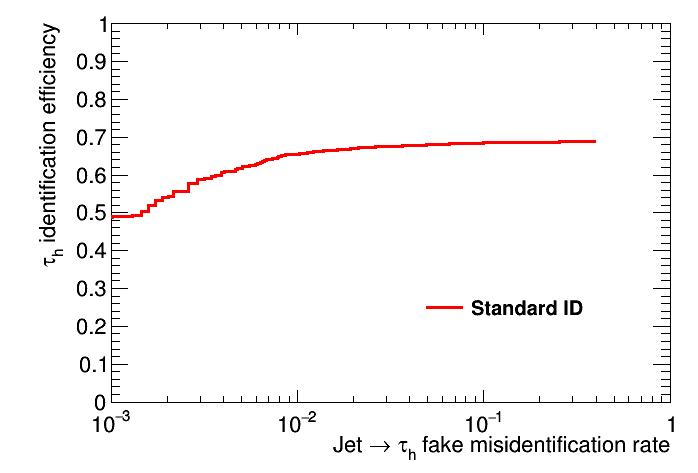
\includegraphics[width=\textwidth]{Images/std_ROC.png}
    \caption{\tauh identification ROC curve for the standard method. The x axis is set to a logarithmic scale.}
    \label{fig:std_ROC}
\end{figure}

Performance are compared in terms of signal efficiency and background rejection. The signal efficiency is defined from the ratio of the number of well-tagged \tauh in the selected population over the total number of \tauh in this population. The background rejection is similarly defined as the ratio of the number of appropriately tagged QCD jets over the total number of QCD jets considered.

While the goal of a classifier is to tag objects as signal or background, most will instead provide with a score between 0 and 1. A score close to 0 is to be interpreted as very likely to be background, and a score close to 1 as very likely to be signal. This continuous score can then be translated into a discrete tag by the choice of a working point (WP) value. For a given WP, every reconstructed jet that scores below the WP value is then tagged as QCD jet, and every reconstructed jet that scores higher than the value a \tauh. The values of the signal efficiency and background rejection can be measured for a continuous scan of WP values, allowing to build a Receiver Operating Characteristic (ROC) curve. The standard identification ROC curve is shown in figure \ref{fig:std_ROC}
Generally, a numerical figure of merit is the area under the ROC curve, called ROC AUC, as it is maximum when signal efficiency and background rejection is perfect.
In our case, ROC AUC might not be the best figure of merit, as it does not take into account which regions are best covered by the technique. Indeed, in our case the standard identification technique is based on applying hard cuts such as decay mode finding and anti-lepton discriminant before evaluating the score of the the isolation BDT. This is why the ROC of the standard technique reaches a plateau, as the plateau corresponds to maximum efficiency allowed by the previous cuts.
QCD jets are also overwhelmingly more present in collisions than \tauh, meaning useful working points are in the region of high background rejection. 

\subsection{Intrinsic limitations}

Both cut-based and BDT-based identification methods rely heavily on designing variables that are likely to have discriminating power, to either create a hard cut directly, or to mix several of these variables into a BDT . But the construction of such variables potentially do not take into account other information that have been gathered in the detection and reconstruction.
While the BDT combines more information than than the cut-based method, it requires fine tuning of the choice of variables. This tuning can lead to a tedious optimization process since the possibilities of information combinations are potentially infinite. Machine learning techniques are intrinsically limited by the amount of information that is available in their inputs. 
A possible improvement should therefore be expected from using a more complete set of variable rather than a selected subset, which is one of the philosophy of deep learning.


\section{From a single neuron to recurrent networks}
\label{sec:NN}
Neural networks are based on combining the principle of a human neuron into networks, using the exponential possibilities of such combination.
They usually require a substantial amount of fully known data as a reference to learn how to perform their given task. The possibility of using simulation allows to have such a substantial  well-known training dataset.
Indeed, neural networks have brought a lot of new results in fields such as big data, image recognition and even pseudo-data generation.

The organization of the neurons in the network is called architecture. The choice of architecture has a strong influence on the training, as neural networks have shown their best achievements through the use of architectures specifically designed for the given task.

\subsection{Basics : neurons, dense networks, deep learning}

\subsubsection{Neuron}

\begin{figure}
    \centering
    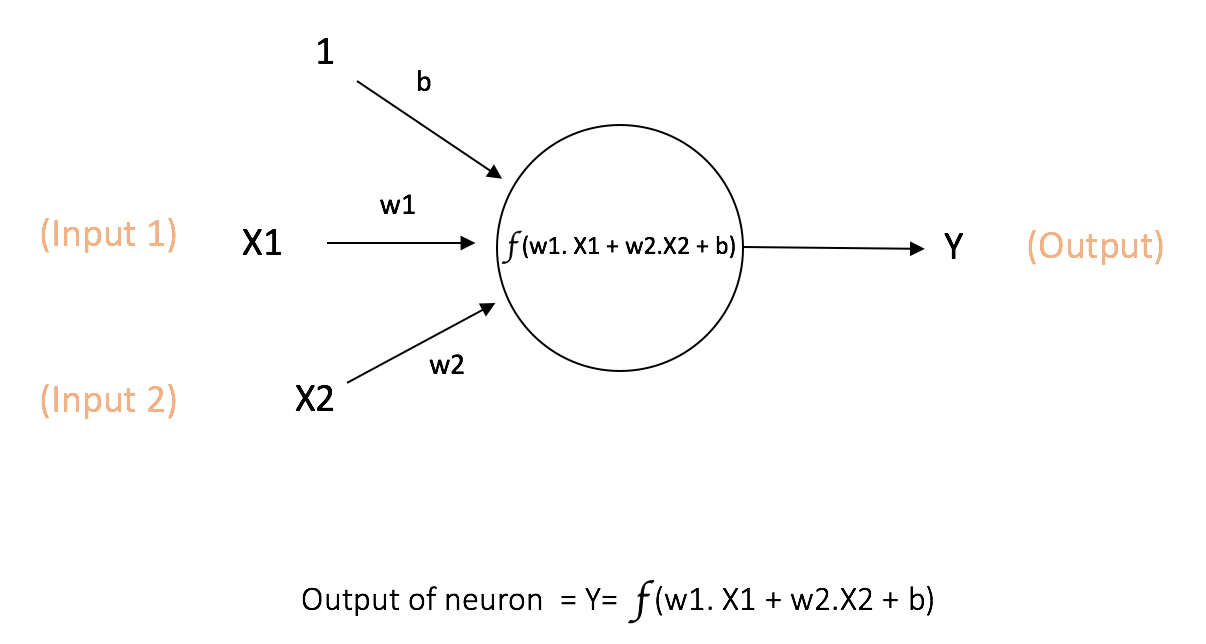
\includegraphics[width=0.8\textwidth]{Images/neuron_diagram}
    \caption{Diagram of a single neuron, in the case of two input variables.}
    \label{fig:neuron_diagram}
\end{figure}


\begin{figure}
    \centering
    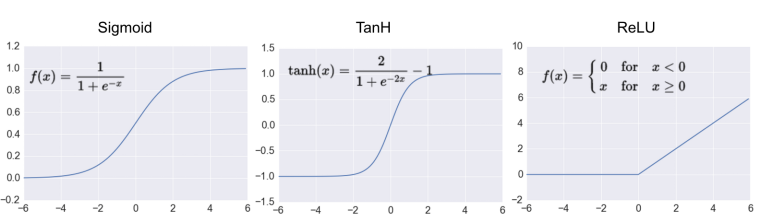
\includegraphics[width=\textwidth]{Images/activation_functions.png}
    \caption{Some activation functions and their visualization.}
    \label{fig:activation_functions}
\end{figure}

A neuron is defined by an activation function $f$, a set of scalar weights $wi$ and a bias $b$. It takes a number of input variables denoted $X_i$ and produces as output the result of $f(\sum w_i\times X_i + b)$. The layout of a neuron is also illustrated in figure \ref{fig:neuron_diagram}. The weighted input is also defined as $z = \sum w_i\times X_i + b$, so that the output of the neuron becomes $f(z)$. The function is called activation function and is chosen among nonlinear differentiable functions. Some examples of widely used activation function are illustrated in figure \ref{fig:activation_functions}. 

\subsubsection{Densely connected network}


\begin{figure}
    \centering
    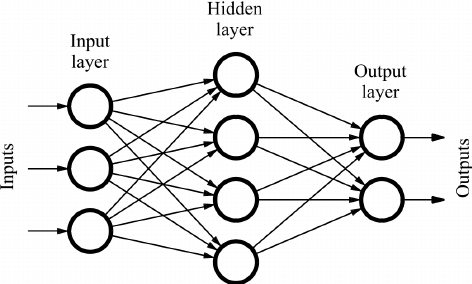
\includegraphics[width=0.5\textwidth]{Images/dense_network.png}
    \caption{Diagram of an example of a feed-forward densely connected network with 3 input variables, 4 neurons in the hidden layer and 2 output neurons.}
    \label{fig:dense_network}
\end{figure}

A network can be created by connecting neurons. A simple case is the feed-forward densely connected network, such as shown in figure \ref{fig:dense_network}. The feed forward nature means that there is no cycle in the propagation of the evaluation from inputs to outputs. In this architecture, neurons are organized by layers, with each neuron's output being an input to each neuron in the next layer. Such organization creates the possibility of approximating theoretically any task as stated by the Universal approximation theorem states \cite{Cybenko1989}, as long as the activation function is non-linear.

\subsubsection{Loss function and backpropagation}

In order to find the set of weights and bias most suited for a task, the network needs to be trained.
The training phase relies on an example set of inputs associated with the target output value. Indeed, the output of the network for a given set of inputs is compared to the target output. This comparison is quantified through the use of a metric called the loss function. The loss function should be a differentiable function of the target value and the output of the network that should be minimum when these variables are equal. Training the network to perform task is therefore equivalent to minimizing the value of the loss function over all possible values for the parameters of the network (weights and biases) for the whole training set.

But the space of configurations of the weights and biases, together called parameters, of the network has a huge dimensionality. The iterative process of training the network can then lead to stagnation if examples are evaluated and parameters adapted for each example of the training set. To avoid this stagnation, the parameters are changed to minimize the average of the loss function over a number of examples, called mini-batch. The number of examples in each mini-batch is referred to as the mini-batch size.

The way the parameters are changed to minimize the loss function depends on which optimizer algorithm is used. Most optimizers rely on backpropagation, meaning the variation that should undergo a parameter is computed by propagating the change of the loss function backwards through all the layers of neurons between the considered neuron and the output of the network. 


A classical problem that can occur in the training of neural networks is the existence of local minima of the loss function. Indeed, local minima can lead to a sub-optimal training, as it prevents the network from reaching a potentially lower global minimum. To mitigate such effects, diminishing learning rates as well as momentum-based optimizers are used. The learning rate is a simple scalar that multiplies the changes in parameters for a given change in loss. By starting at a high value of this learning rate, it is possible to avoid local minima that are too small, while in later stage of the training, this rate can be lowered to help reach the lowest point of the minimum. Momentum-based optimizers try to avoid momentum by accelerating the learning rate by a factor proportional to the size of the last step. Indeed, the more a training step helped minimizing the loss function, the bigger the next step, avoiding local minima on the way to a global minimum.

Backpropagation comes with another important problem called vanishing gradients. This roughly is due to output of layers being generally relatively small compared to the input of a neuron. Indeed, an activation function such as the sigmoid, illustrated in figure \ref{fig:activation_functions}, can be lead to states where the derivative is close to 0. Since backpropagation finds the derivatives of the cost function with respect to the parameters by using the chain rule backward from the last layer. This means the more layers are in between a neuron and the final layer, the more chance that its parameters will update based on the derivative that is likely close to 0. In other words, this also means that a change in the parameters of a neuron in an early layer will have a relatively small effect on the loss compared to a similar change in the late layers. In the training, this leads to a slower training of the early layers compared than the last layers. Therefore, a very deep network, meaning many layers, will overall need a lot bigger training set and also a longer training time. This can be mitigated by the use of activation function such as the ReLU, which is defined as $f(x)=0$ for $x < 0$ and $f(x)=x$ for $x \geq 0$ as illustrated in figure \ref{fig:activation_functions}. This activation function avoids the small derivative by not requiring its output to be between 0 and 1. The use of cross-entropy as a loss function also allows to mitigate the vanishing gradients problem, as the derivative of the activation function cancels out in the computation of the overall derivative of the cost function with respect to the parameters \cite{NN_book}. One can also mitigate further this problem by designing an architectural workaround, avoiding deep network when possible, for example using recurrent neural networks, which are introduced in the following section.

    % \begin{equation}
    %     L = \frac{1}{n} \sum_x L_x
    % \end{equation}
    % \item (base explanation same way as http://neuralnetworksanddeeplearning.com/chap2.html and cite!)
    % \item notation : 
    % \begin{itemize}
    %     \item $w_{jk}^{l}$  denote the weight for the connection from the $k^{th}$ neuron in  the $(l-1)^{th}$ layer to the $j^{th}$ neuron in the $l^{th}$ layer and $b_{j}^{l}$ the bias of the $j^{th}$ neuron in the $l^{th}$ layer
    %     \item $\sigma$ is the activation unction
    %     \item $a_{j}^{l}$ is the activation of the $j^{th}$ neuron in the $l^{th}$ layer
    %     \item therefore 
    %     \begin{equation}
    %         a_{j}^{l} = \sigma \Big( \sum_k w_{jk}^{k}a_{k}^{l-1} + b_{j}^{l} \Big)
    %     \end{equation}
    %     \item to lighten the scripture, let's use the vectorized form:
    %     \begin{equation}
    %         a^l = \sigma \Big( w^l a^{l-1} + b^l \Big)
    %     \end{equation}
    %     \item with
    %     \begin{equation}
    %         f\begin{pmatrix} x_1 \\ x_2 \end{pmatrix} = \begin{pmatrix} f(x_1) \\ f(x_2) \end{pmatrix}
    %     \end{equation}
    %     \item also to lighten the scripture let's define :
    %     \begin{equation}
    %         z_j^l = \sum_k w^l_{jk} a_k^{l-1} + b_j^l
    %     \end{equation}
    %     \item and
    %     \begin{equation}
    %         (s \odot t)_j = s_j t_j
    %     \end{equation}
    %     \item now let's define the "learnability" (good word?) of neuron $j$ in the $l^th$ layer:
    %     \begin{equation}
    %         \delta_j^l \equiv \frac{\partial L}{\partial z_l^j}
    %     \end{equation}
    % \end{itemize}
    % \item problem : local minimas
    % \item part of the solution : momentum
    % \item further solution : ADAM
    % \item problem : vanishing gradient
    % \item part of the solution : right choice of loss function (cross-entropy)


\subsection{Recurrent neural networks}

\begin{figure}
    \centering
    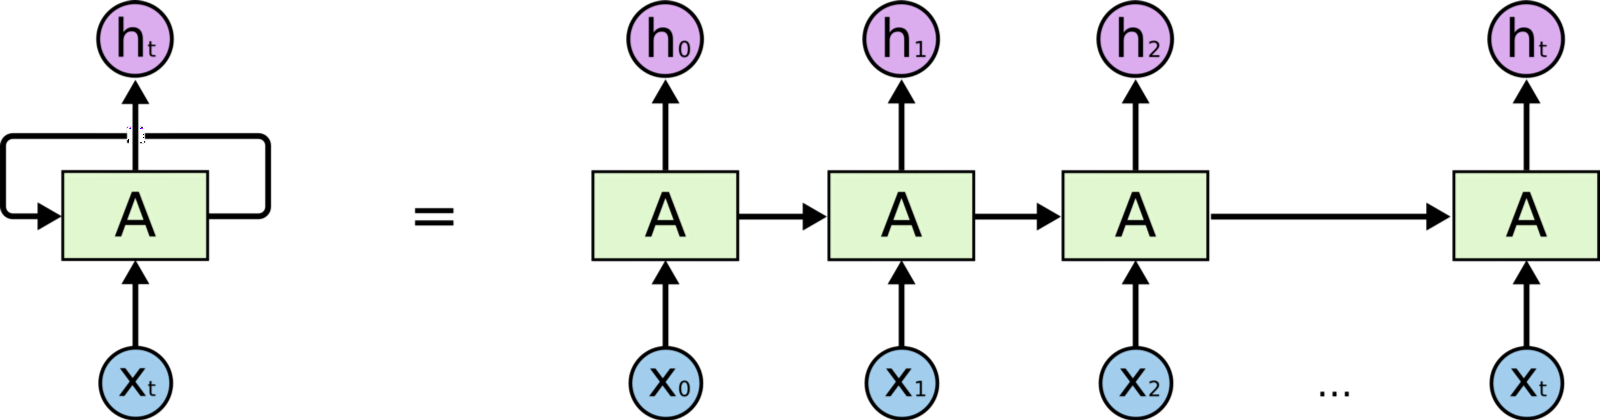
\includegraphics[width=\textwidth]{Images/recurrent_network.png}
    \caption{Diagram of the evaluation of a recurrent network on successive sets of inputs from \cite{RNN}.}
    \label{fig:recurrent_network}
\end{figure}

Recurrent neural network have been designed to fit the necessities of language processing, which are in some extent similar to the \tauh identification of reconstructed jets. Indeed, the information is delivered in sentences, which are a set of words with a varying length, which can be assimilated to a jet, which is a set of particle with a varying length. Classical neural networks, such as the densely connected network, have a fixed number of input variables, which makes them unable to process such information as it is. To fit this information format, recurrent networks work by iteration over each word. The same network will be evaluated iteratively on each word, while giving a channel of communication with its next evaluation, as illustrated in figure \ref{fig:recurrent_network}. The communication channel with its next iterations takes the form of a secondary output to the network that feeds into a secondary input at the next iteration. In most cases, only the last iteration of the primary output of the layers is considered as the final output of the network. The secondary communication channel between iteration can be interpreted as an inner representation of the inputs that builds up at each iteration, before being used in the final output.

This architecture can be interpreted as dividing the inner working of the network into two parts. A first part has the role of building up the inner representation at each iteration, while a second part is only evaluated at the last iteration in order to produce the desired output from the inner representation. An important feature is that the first part of the channel is the same at each iteration, meaning the total number of independent parameter is kept low. By designing such an architecture, one of the goals is to separate a complex task into a subset of two other simpler tasks, allowing the task to be fulfilled by a less deep network, avoiding the vanishing gradient problem.

\section{Recursive neural network}
\label{sec:RecNN}
Neural network architectures should fit the format of the input while providing an information flow as adapted as possible to the task at hand. This recursive neural network (RecNN) architecture is used to perform the task of correctly identify \tauh decay products from a set of reconstructed jets, with QCD jets as the main background. Such an architecture based on the jet structure was developed in order to separate boosted W-jet from QCD jets \cite{Louppe:2017ipp}. The architecture is chosen to be based on the jet clustering algorithms. We will detail the adaptation of such idea to our case as well as different improvements that were implemented.

\subsection{Base architecture}

\begin{figure}
    \centering
    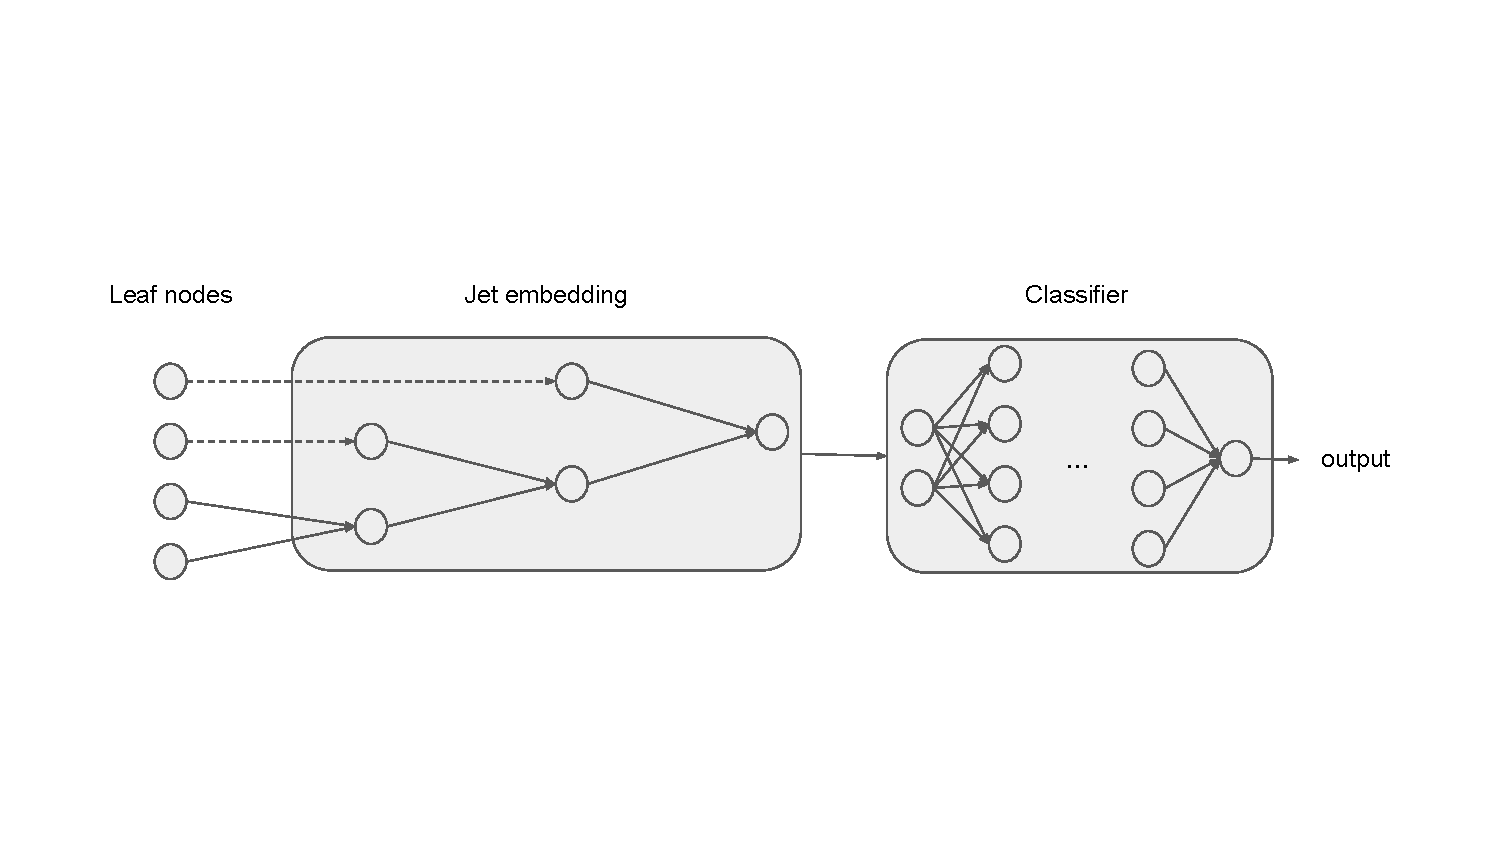
\includegraphics[width=\textwidth]{Images/RecNNdiagram.pdf}
    \caption{Nodal architecture of a Recursive neural network (RecNN).}
    \label{fig:recnn_architecture}
\end{figure}

\begin{figure}
    \begin{center}
    \subfloat[RecNN leaf node]{
        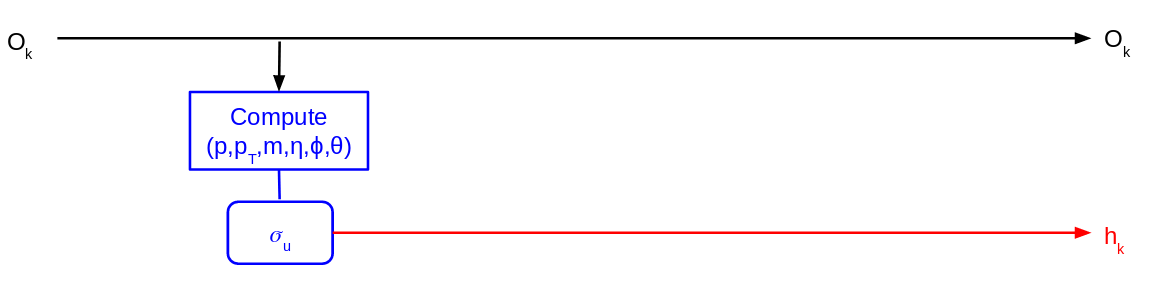
\includegraphics[width=\textwidth]{Images/simpleRecNN.png}
        \label{sub:RecNNLeafNode}
    }
    
    \subfloat[RecNN node]{
        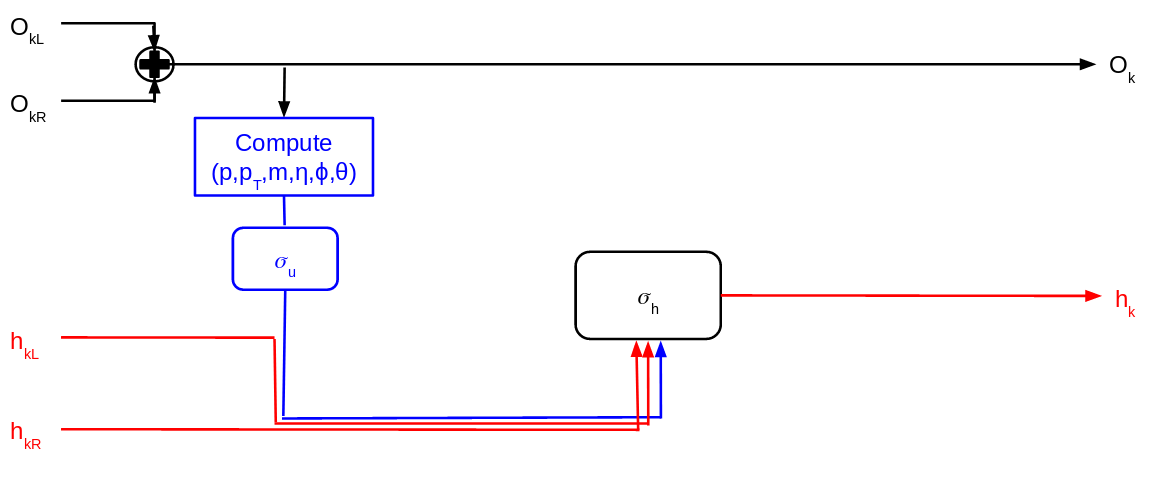
\includegraphics[width=\textwidth]{Images/simpleRecNN2.png}
        \label{sub:RecNNNode}
    }
    
    \subfloat[Gated RecNN node]{
        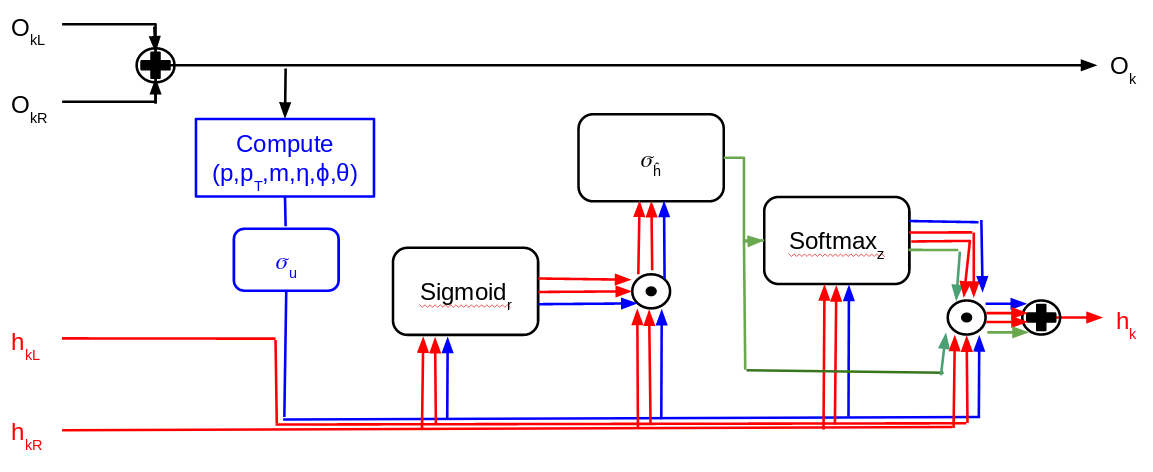
\includegraphics[width=\textwidth]{Images/gatedRecNN.png}
        \label{sub:GatedRecNNNode}
    }
    
    \caption{Diagrams of different nodes that can be found in a RecNN architecture. Top is a leaf node, middle is a non-leaf node. Bottom is a non-leaf node for a gated RecNN architecture.}
    \label{fig:recnn_nodes}
    \end{center}
\end{figure}

The network architecture will be divided into two parts, similarly to the recurrent architecture. A first embedding part is organized from a jet clustering structure. Its output then fed to a dense feed-forward network architecture, as illustrated in figure \ref{fig:recnn_architecture}.
The jet-embedding part is built as an ensemble of nodes. Similarly to recurrent networks, the neuron layers in each node have the same parameters. Also similarly to the word-based scheme in recurrent network, the recursive network is particle-based, meaning the input jet is broken down to its constituent particles, and each particle is fed into an input node, called leaf-node. To build the jet-embedding structure, two nodes are selected using a chosen metric, and feed into a new node, iteratively, until there is only one node left. 
The metric used to select which nodes are to be merged can be chosen among the following set:
    
\begin{itemize}
    \item randomized : two nodes are selected at random
    \item pt-ordered : the nodes holding the two pseudo-particles with the highest pt 
    \item reversed pt-ordered : the nodes holding the two pseudo-particles with the lowest pt
    \item kt : nodes holding closest pseudo-particles following the kt clustering metric
    \item Cambridge : nodes holding closest pseudo-particles following the Cambridge clustering metric
    \item anti-kt : nodes holding closest pseudo-particles following the anti-kt metric
\end{itemize}
The distance of two particles $i$ and $j$ is defined as
\begin{equation}
    d_{ij} = \mathrm{min}(p_{Ti}^{2k},p_{Tj}^{2k}) \frac{\Delta_{ij}}{\mathrm{R}} \mend
\end{equation}
In this expression $\Delta_{ij}$ corresponds to the distance of the particles in the ($\eta$,$\phi$) plane, R is a distance parameter, and $p_{Ti}^{2k}$ corresponds to the modulus of the transverse momentum of particle $i$, with the $k$ parameter being equal to 1 for the kt metric, 0 for the Cambridge metric, and $-1$ for the anti-kt metric.

In the jet embedding part, the information takes two distinct paths, as illustrated in figure \ref{fig:recnn_nodes}.
The vector $O_k$ was originally the 4-momentum of the pseudo-jet at the node k in the original design. It has been upgraded to hold extra information in the new version. First, The 4-momentum is split by particle type : photon, electron, muon, charged hadron, neutral hadron. This is done to allow the network to base its decision on the types of particles rather than just the overall 4-momentum. Second, the 4-momentum vector is also concatenated with information on each subjets. As the $O_k$ vector is computed as the sum of the $O_{kl}$ and $O_{kr}$ vectors, coming from the nodes that were merged into node $k$, the new information must be addable. The chosen extra variables are the total charge and total number of particles for each type constituent. On top of this, the distance in the ($\eta$,$\phi$) plane between the merged pseudo-jets is fed to the network at each successive step of the clustering. 

At each node a full set of variables is also re-computed from the 4-momenta : p, \pt, m, $\eta$, $\phi$, $\theta$. All of these variables are then fed into a neuron layer called $\sigma_{u}$ instead of the 4-momentum in Cartesian form.
On a leaf node k, the output of $\sigma_{u}$ is then taken as the embedded output of this node, named $h_k$.
On a non-leaf node k, the output of $\sigma_{u}$ is fed along the embedded outputs of the previous layers into another layer, namely $\sigma_h$. the output of $\sigma_h$ is then the embedded output $h_k$.
Effectively there are indeed two paths for the information in the architecture: a direct pseudo-particle like clustering where 4-momentum and addable characteristics are added, and a path where neuron layers embed the information and mixes it with the existing previously embedded information.

\subsection{Gating}

Gated RecNN adds an extra complexity on the scheme of layers in a node, as illustrated in figure \ref{fig:recnn_nodes}. Inspired by the long short-term memory (LSTM) architecture \cite{lstm}, the gating adds the possibility for the network to select and mix information in the embedding scheme more easily. 

A new neuron layer $\mathrm{Sigmoid}_r$, takes 3 input vectors : $h_k_l$,$h_k_r$ and the output of layer $\sigma_u$. It will give 3 scalar outputs that will be used to multiply the same vectors respectively. Each multiplied vector is then fed into layer $\sigma_\hat{h}$. 
The four vectors $h_k_l$, $h_k_r$, output of $\sigma_u$ and output of $\sigma_\hat{h}$ are going to be weighted and added. The weights $w_i$ are determined by another neuron layer called $\mathrm{Softmax}_z$. The output of $\mathrm{Softmax}_z$ are forced to respect the following equations :
\begin{equation}    
    h_{k} = \sum_{n_{i}=h_{kL},h_{kR},u,\hat{h}} w_{i}n_{i}
\end{equation}
\begin{equation}
    w_{i} = \frac{e^{Z_i}}{\sum_{j=1}^{K}e^{Z_j}}
\end{equation}
This will allow the network to easily choose to enhance certain information paths and belittle information paths that seems not to be useful.

\subsection{Pre-processing}

In order to simplify the task, jets are de-boosted and centered using the highest \pt particle, meaning particles appear orientated around the center (0,0) of the ($\eta$,$\phi$) plane. The jet is then re-clustered into three subjets and rotated and/or mirrored so that the general disposition of subjets are similar. This is done in order to simplify the task for the network.

Another issue arise from the distribution of signal and background jets in the training sample. If both background and signal samples had different \pt distribution, the network could wrongly assume that the \pt of a reconstructed jet is correlated to the identification task. To avoid statistical this bias in the training samples, the signal and background jets are selected for many \pt bins, in order to have the same number of signal and background events in each bin.

\subsection{Implementation}

While most neural network architecture can easily be implemented using available libraries, the RecNN architecture had to be implemented by hand using base classes from the sklearn library \cite{scikit-learn}. This is due to the architecture being adapted to each jet following the clustering algorithm applied to the considered jet. Therefore, using the implementation shared by the original article \cite{Louppe:2017ipp} as a base, many featured had to be re-implemented. For example, the fastjet \cite{Cacciari:2011ma} clustering algorithm interface had to be re-made in order to match the changes brought to the code, for example the matching of pseudo-jets to their respective extra information. Also the pre-processing and clustering evaluation steps have been reshaped to use multithreading, allowing faster computational times. Some libraries were changed to maximize computational efficiency, such as the disk writing format.

A major upgrade that was implemented was related to trackability of the jets. Indeed, once the jet was pre-processed and re-clustered, the link with related information not involved in the network was lost. Once this feature was implemented, populations defined by the performance of both standard and RecNN methods could be studied on a broader level. A jet display was also implemented to study jets on a case-by-case basis. This jet-by-jet study allowed to understand the shortcomings of the network and design new features to avoid them.

A feature that was mostly recovered from the original paper with minor changes was the parallelisation of tree evaluation and training computing steps. To implement this parallelisation, parameters are evaluated, or trained, simultaneously across each node depth level for multiple jets at a time, as illustrated in \ref{fig:RecNN_parall}. While this allows to gain time computationally, it adds a level of complexity to the whole structure of the code, as the neuron parameters are concatenated across node depth for several different jets at a time.

\begin{figure}
    \centering
    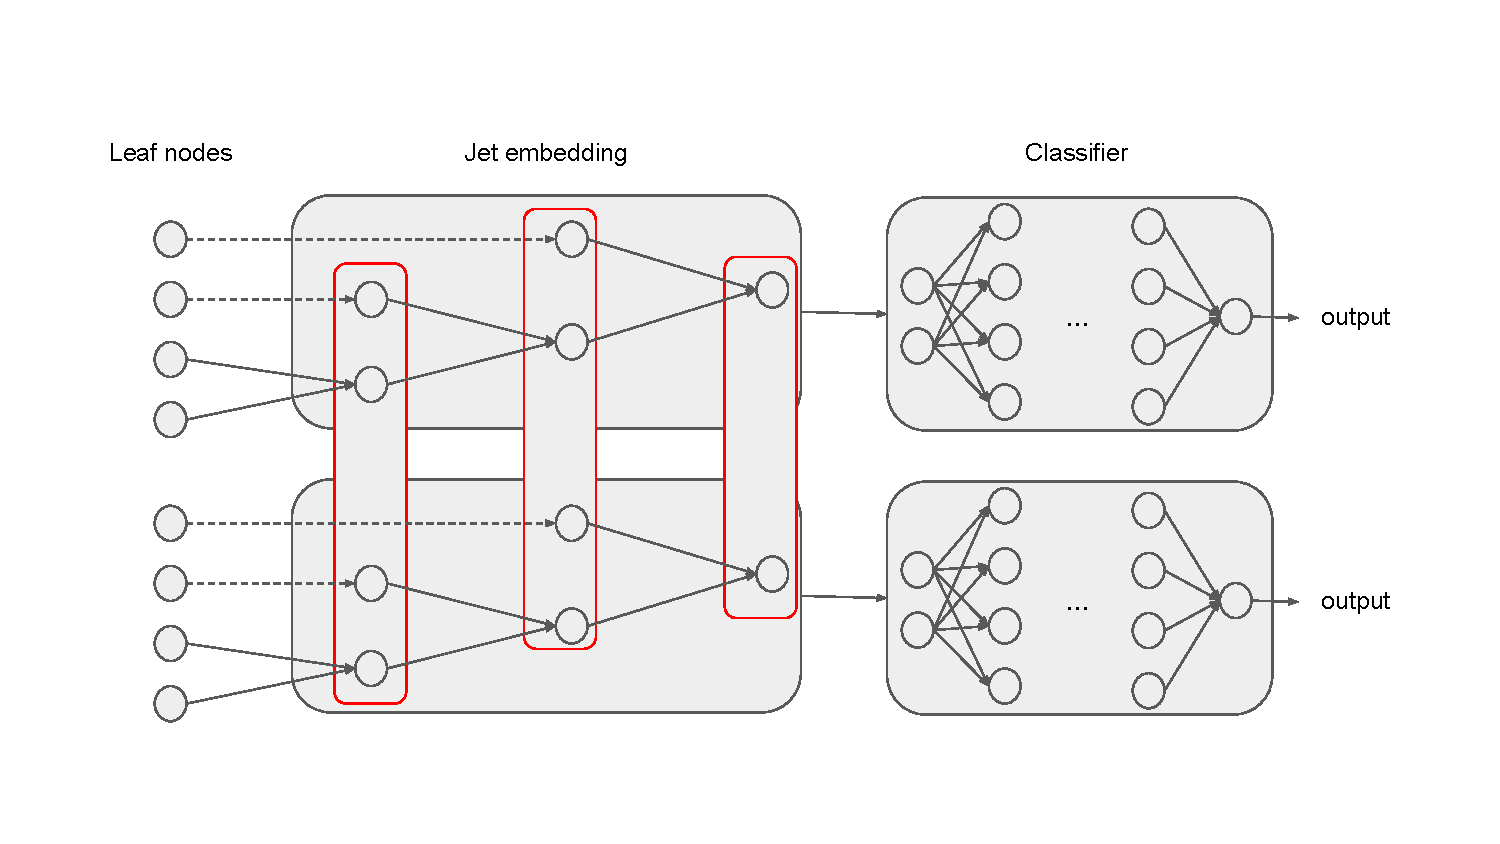
\includegraphics[width=\textwidth]{Images/RecNN_diagram_parall.pdf}
    \caption{Illustration of the parallelisation of computing in the RecNN. The red boxes correspond to node-depth levels that are evaluated and trained parallely.}
    \label{fig:RecNN_parall}
\end{figure}

\subsection{Performance}

\begin{figure}
    \centering
    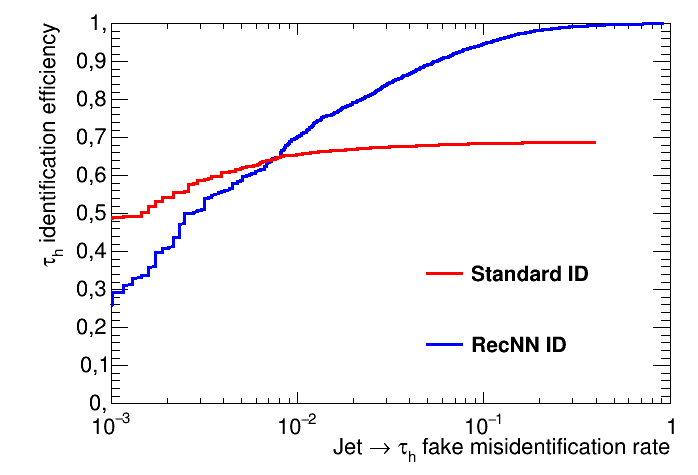
\includegraphics[width=\textwidth]{Images/ROC_comp.png}
    \caption{\tauh identification ROC curve for the standard method and with the RecNN method. The x axis is set to a logarithmic scale.}
    \label{fig:RecNN_ROC}
\end{figure}

Even while limiting as much as possible the computational times, the later versions of the networks have proven to be long to train. Hyper-parameters are the overall parameters of the network, not to be mixed with each neuron parameters. The hyper-parameters of our network can be whether to use the gated scheme or not, the number of layers in a given part of the network, the number of neuron in each of the layer, the clustering order used to shape the embedding part of the network, the choice of loss function, optimizer and activation function for each neuron... The lengthy training times combined with the number of hyper-parameter meant that this study can't provide with the best version of our chosen architecture, but instead aims to show proof of concept.

All the clustering orderings have shown similar results in several stages of optimization. While all should be tested in an optimization study, the presented results have been produced with the anti-kt ordering. Also, at all stages the gated approach has lead to far better results than the non-gated, leading to the non-gated not being studied further.

The ROC curves of both the standard method and the best found RecNN approach are presented in figure \ref{fig:RecNN_ROC}. While the area under the curve is strictly better in the RecNN approach, the efficiency of the standard method is still better at low jet misidentification rate. The working points used in the CMS analysis are around 60$\%$ identification efficiency, not far from where the curves cross. But the RecNN approach allows to reach far better QCD jet rejection at high \tauh efficiency.

\subsection{Possible optimization}

Although the results have shown some potential, this study has not reached the level of optimization that could help the RecNN to outperform the standard technique. Indeed, several upgrades that could benefit the RecNN approach have been considered, but where not fully implemented in time. 

One such upgrade idea come from the study of QCD jets misidentified by the RecNN. Indeed, many examples such as the one displayed in figure \ref{fig:jet_display} show that the RecNN approach does not use the number of particle information as efficiently as it could. An upgrade would be to directly add the number of particle per type at the classifier-level, rather than the jet embedding level. This could help the network to easily reject trivial cases, while being able to specialize the jet-embedding part for the less straight-forward cases.

Another upgrade could be the use of subset in the training. Indeed, a majority of training cases are trivial, meaning most of the cases will not help the network to learn classify the difficult cases, but instead overtrain. Overtraining is the effect happening when the features that are learnt are specific to the sample and not applicable to the general task. The training of such machine learning algorithm is usually stopped as soon as this overtraining appears. To do so, a separate independent sample is used to evaluate the network's performance. Overtraining is declared when the performance on the independent sample starts degrading while the performance computed on the training samples keeps upgrading.

\begin{figure}
    \centering
    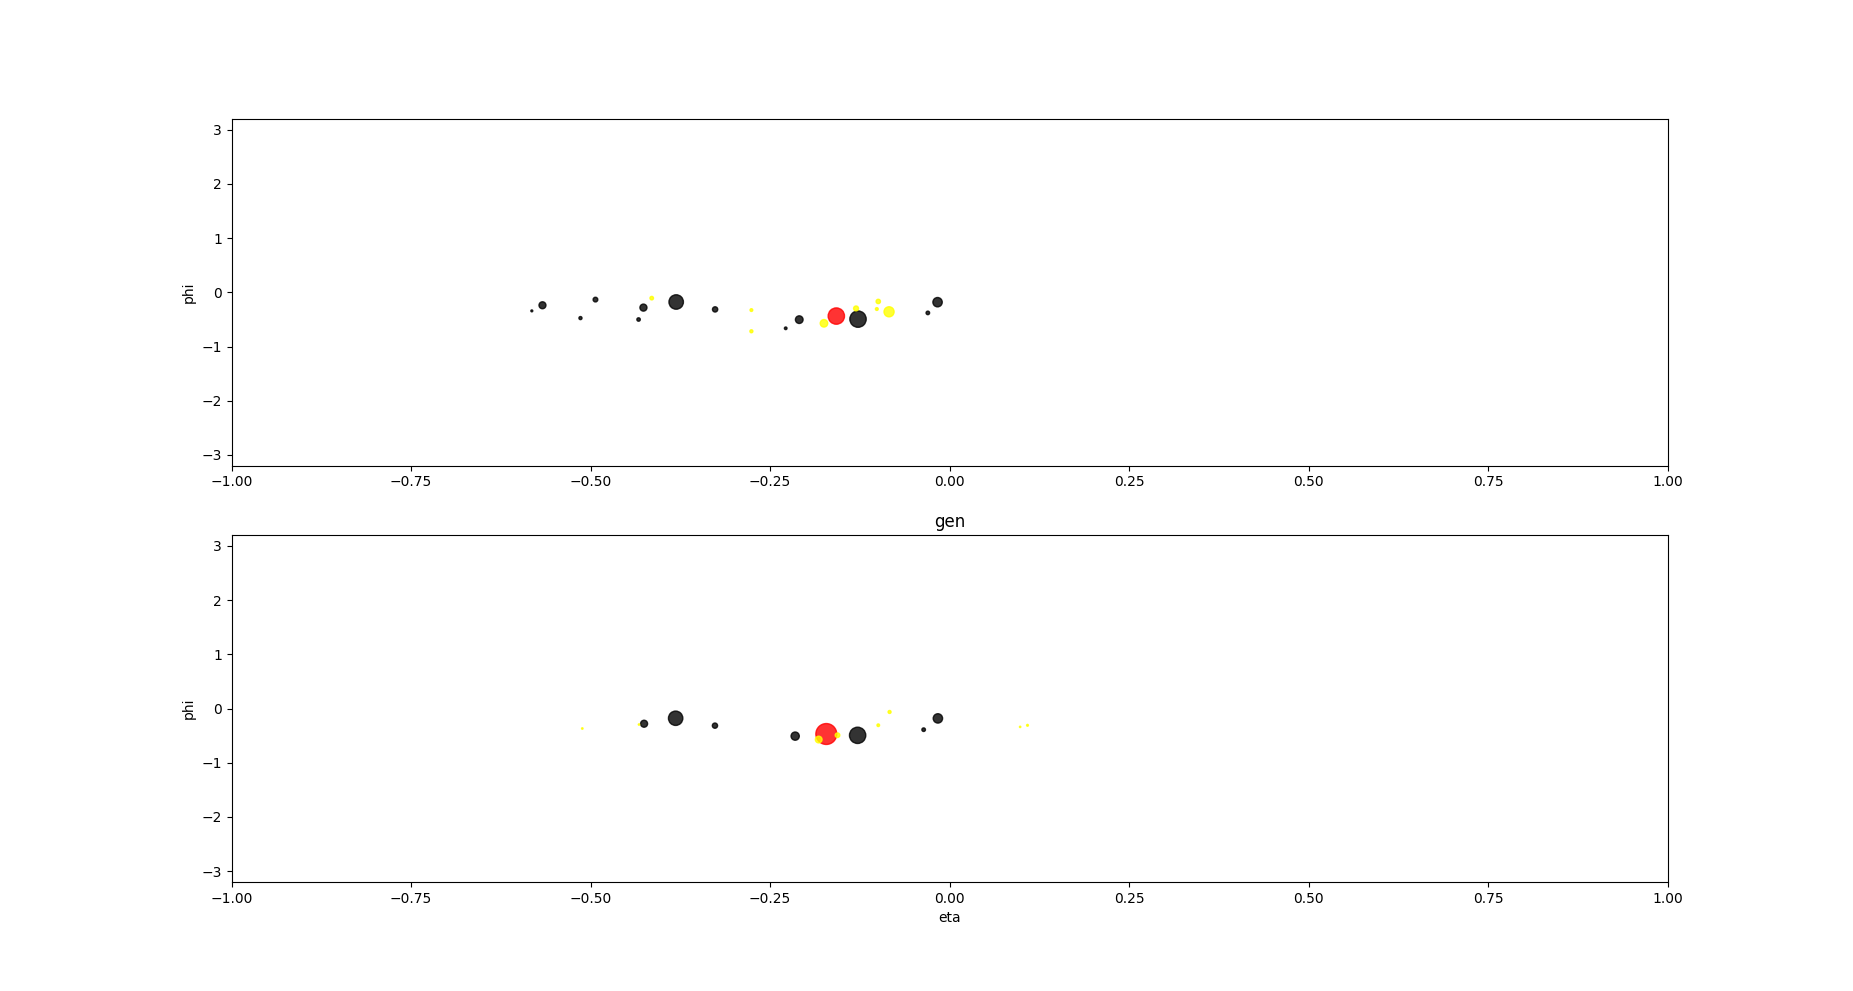
\includegraphics[width=\textwidth]{Images/jet_display1.png}
    \caption{Scatter plots of the constituents in a QCD jet misidentified by the RecNN network. Top plot is the reconstructed jet, and the bottom plot is the gen-level jet. The size of the points are proportional to their \pt and their color depends on their type. Black is a charged hadron, yellow is a photon and red is a neutral hadron.}
    \label{fig:jet_display}
\end{figure}
